\documentclass[journal]{IEEEtran}
\usepackage{cite}
\usepackage{amsmath,amssymb}
\usepackage{graphicx}
\usepackage{booktabs}
\usepackage{multirow}
\usepackage{algorithm}
\usepackage{algpseudocode}
\usepackage{tikz}
\usetikzlibrary{positioning,arrows.meta,fit}
\usepackage[hidelinks]{hyperref}
\renewcommand{\algorithmicrequire}{\textbf{Input:}}
\renewcommand{\algorithmicensure}{\textbf{Output:}}
\newcommand{\pmv}[2]{#1{\scriptsize$\pm$#2}}
\usepackage{xcolor}
% Revised text is blue. For the clean version, compile main_clean.tex (defines \cleanversion).
\ifdefined\cleanversion\newcommand{\rev}[1]{#1}\else\newcommand{\rev}[1]{{\color{blue}#1}}\fi
\newcommand{\pms}[2]{#1{\tiny$\pm$#2}}

\begin{document}

\title{EASFL: Energy-Aware Federated Anomaly Detection in Wireless Sensor Networks With Mask-Aware Robust Aggregation}

\author{Shiva~Kumar~V
and~Choupiri~Shivakeshi
\thanks{Shiva Kumar V (corresponding author) and Choupiri Shivakeshi are with the Department of Computer Science and Engineering, Kishkinda University, Ballari, Karnataka, India (e-mail: shivakumar@kishkindauniversity.edu.in; shivakeshic@kishkindauniversity.edu.in).}}

\markboth{IEEE Internet of Things Journal}{Shiva Kumar V and Shivakeshi: EASFL for Anomaly Detection in WSNs}

\maketitle

\begin{abstract}
Federated learning (FL) keeps raw sensor data on the nodes of a wireless sensor network (WSN), but exchanging model updates over low-power radios can drain batteries faster than shipping the raw data. We present EASFL, a cluster-based FL framework for on-node anomaly detection that treats energy as a first-class constraint. EASFL combines energy-aware cluster-head and participant selection, top-$k$ sparsified 8-bit updates with error feedback, two-tier robust aggregation with reputation-based quarantine, and zero-communication on-node personalization. \rev{Its mask-aware aggregation (EASFL-M) compares sparsified updates only on the coordinates they carry, so that honest nodes are not mistaken for attackers.} We also introduce a network-level F1-score in which depleted nodes raise no alarms. In a 100-node simulation with a synthetic workload, EASFL cuts traffic by $13\times$ and energy by $3\times$ relative to hierarchical FedAvg, delays the first node death from round 35 to 547, and attains a network-level F1-score of 0.82 at round 200 against 0.26, while keeping F1 within 0.07 of its clean value under four poisoning attacks with up to 20\% malicious nodes. \rev{In a semi-synthetic validation that uses the real readings and layout of the 50-mote Intel Lab deployment with injected faults,} EASFL keeps every node alive to round 200, uses $16\times$ less traffic and $3.3\times$ less energy, matches the per-node F1 of hierarchical FedAvg (0.56), and raises network-level F1 from 0.32 to 0.57. \rev{Against baselines given the same compression and participation, mask-aware aggregation resists sign-flip poisoning significantly better on both data sets.}
\end{abstract}

\begin{IEEEkeywords}
Wireless sensor networks, federated learning, anomaly detection, energy efficiency, network lifetime, clustering, model poisoning, non-IID data, personalization.
\end{IEEEkeywords}

\section{Introduction}
\IEEEPARstart{W}{ireless} sensor networks (WSNs) underpin environmental, structural and industrial monitoring in the Internet of Things (IoT). Their readings are routinely corrupted by spikes, stuck-at values, drifts and noise bursts caused by failing hardware, depleted batteries, environmental extremes or tampering~\cite{ni2009,sharma2010}, and detecting such anomalies close to the source is essential for data quality and security~\cite{rajasegarar2008}. The conventional approach forwards raw readings to a base station (BS) for centralized learning. This exposes potentially sensitive data, adds latency and, crucially for battery-powered nodes, spends scarce energy on bulk transmission.

Federated learning (FL)~\cite{mcmahan2017,kairouz2021} offers an alternative: nodes train locally and share only model updates. FL has been applied to IoT anomaly and intrusion detection~\cite{nguyen2019diot,mothukuri2022}, but most work assumes edge devices with stable power and connectivity~\cite{lim2020}. In a WSN, three problems remain. First, \emph{communication energy}: every round moves a full model from every participant, so naive FL can exhaust the network faster than centralized collection (Section~\ref{sec:results}). Second, \emph{heterogeneity}: each node sees its own environment and fault mix, so data are non-IID and a single global model under-fits individual nodes~\cite{zhao2018,hsu2019}. Third, \emph{trust}: nodes are physically exposed, and a few compromised nodes can poison the shared model~\cite{blanchard2017,fang2020,uddin2025}. Recent WSN studies combine two of these concerns, for example energy-aware client selection with sparsified updates and trust-weighted aggregation~\cite{bhagyalakshmi2026}, or energy-aware participation with model compression for routing~\cite{hawkinson2025}. They report accuracy and energy separately, however, and rarely show how learning choices change node deaths, or how a network that is losing nodes to battery exhaustion detects anomalies.

This paper proposes EASFL, an energy-aware, poisoning-resilient FL framework that addresses all three jointly within the clustered architecture already standard in WSNs~\cite{heinzelman2002,younis2004,abbasi2007}. Our contributions are:
\begin{enumerate}
\item A cluster-based FL protocol whose every component (head selection, participant selection, update compression, aggregation) is chosen to reduce radio energy, with an explicit bit-level cost model.
\item \rev{A mask-aware two-tier robust aggregation rule (EASFL-M) with reputation-based quarantine that requires no trusted root dataset. Its direction filter and trimmed mean act only on the coordinates each top-$k$ sparsified update carries, so Byzantine-robust aggregation works on compressed updates without discarding honest ones.} A zero-communication on-node personalization step completes the framework.
\item A reproducible evaluation with energy-coupled detection metrics, including a \emph{network-level} F1-score in which nodes that have exhausted their batteries raise no alarms, ablations, four attack models against \rev{five robust-aggregation baselines that use the same compression, participation and cluster-head policy as EASFL (20 seeds, paired significance tests), detection quality over the whole network lifetime,} sensitivity analyses of the synthetic workload, and a validation on real readings and the real layout of the Intel Berkeley Lab deployment. All code and seeds are publicly released.
\end{enumerate}

\section{Related Work}
\textit{Energy-efficient clustering and FL in WSNs.} LEACH~\cite{heinzelman2002} rotates cluster heads (CHs) randomly to spread load, and HEED~\cite{younis2004} uses residual energy and communication cost; see~\cite{abbasi2007} for a survey. These protocols target data gathering. More recent work couples clustering with learning: Baqer~\cite{baqer2025} integrates a hierarchical clustering routing protocol with FL to reduce the number of communication rounds, and FLAR~\cite{hawkinson2025} combines energy-aware participant selection and adaptive model compression to extend WSN lifetime in an FL-based routing scheme. In our earlier work, PRO:GED\_DQN~\cite{shivakumar2026gossip} selects gossiping next hops by residual energy, entropy and node degree and trains a deep Q-network routing model with FL in resource-constrained WSNs. These works use FL to improve routing; EASFL instead uses it to train the anomaly detector itself and makes the learning protocol, rather than the routing layer, energy-aware and robust to poisoning. EASFL also reuses the clustered structure, but it selects heads and participants for the FL workload itself and evaluates the result as an anomaly detector.

\textit{Communication-efficient and energy-aware FL.} Sparsification with error feedback~\cite{lin2018dgc,stich2018} and sparse ternary compression~\cite{sattler2020} reduce upload volume, and adaptive sparsification and quantization~\cite{marnissi2024,compaore2025,zhu2025} tune compression to the energy budget of IoT devices. Client selection accounts for heterogeneous resources~\cite{nishio2019}, and recent schemes select or sample clients by energy in hierarchical and IoT settings~\cite{trindade2024,trindade2026,yang2025symbiotic}. Hierarchical client--edge--cloud aggregation cuts long-haul traffic~\cite{liu2020hfl}, adaptive aggregation frequency trades computation for communication~\cite{wang2019adaptive}, and decentralized designs remove the central server~\cite{taherijavan2025}; see~\cite{yan2024survey} for a survey. Barbieri \textit{et al.}~\cite{barbieri2025} quantify the energy and carbon footprint of robust FL, including the effect of quantization and sparsification. Most of these works target edge devices and measure cost in bytes, latency or total energy. We measure it in joules under a WSN radio model and report its effect on individual node deaths.

\textit{Robust FL and heterogeneity.} Byzantine-robust rules include Krum~\cite{blanchard2017}, coordinate-wise median and trimmed mean~\cite{yin2018}, and FLTrust, which requires a clean root dataset at the server~\cite{cao2021}. Adaptive attacks~\cite{fang2020} and backdoors~\cite{bagdasaryan2020} show that no single rule suffices~\cite{uddin2025}. For IoT, FLOW~\cite{liu2024flow} filters updates by cosine distance using current and historical rounds, and Hu \textit{et al.}~\cite{hu2024} measure cosine similarity directly on compressed updates; reputation-based consensus~\cite{rashid2025} weights clients by their past behaviour. EASFL's direction filter and quarantine follow the same principles but run in two tiers, at the CH and at the BS, on sparsified and quantized updates. For non-IID data, proximal regularization (FedProx)~\cite{li2020fedprox} and personalization~\cite{arivazhagan2019,tan2023} are common, and recent work combines personalization with poisoning defence~\cite{cao2024,thein2024,sun2025}. Cryptographic secure aggregation~\cite{bonawitz2017} protects update confidentiality but not integrity and is orthogonal to our design.

\textit{FL for sensor and IoT anomaly detection.} D\"IoT~\cite{nguyen2019diot} and~\cite{mothukuri2022} detect compromised IoT devices with FL, and communication-efficient on-device FL has been applied to industrial time-series anomaly detection~\cite{liu2021jiot}; on-board training on microcontrollers is now feasible~\cite{ficco2024}. These works target gateways or mains-powered devices and do not model radio energy or lifetime. In sensor networks, FL has been used for ensemble online anomaly detection with cloud aggregation~\cite{gayathri2024}, for threat detection~\cite{gupta2025}, and for lightweight environmental monitoring with energy-weighted aggregation of detection thresholds~\cite{yan2024lsens}. Closest to our work, Bhagyalakshmi \textit{et al.}~\cite{bhagyalakshmi2026} combine a CNN--GRU detector, trust-weighted server-side aggregation, top-$k$ sparsification and client selection based on energy level, network lifespan and link quality for WSN anomaly detection on the WUSTL and Intel Lab data, and evaluate accuracy, convergence and robustness to unreliable connections and noise. TEA-FL~\cite{reis2026} guides client participation and aggregation jointly by residual energy and trust scores in WSN settings, evaluated on proxy activity-recognition and intrusion-detection benchmarks, and its authors note that it is not a complete Byzantine-robust defence. EASFL differs from both in four respects: it uses a clustered two-tier architecture and selects CHs as well as participants by residual energy; it evaluates the defence against explicit model- and data-poisoning attacks rather than dropout and noise; it personalizes the detector on each node without extra communication; and it reports the outcome as node deaths (FND, HND, LND) under a bit-level energy model, together with a network-level F1-score in which dead nodes raise no alarms.

\section{System Model}\label{sec:model}
\subsection{Network and Energy Model}
$N$ static nodes are deployed uniformly in an $L\times L$ field with a BS outside the field. Node $i$ starts with heterogeneous energy $E_i^0\sim\mathcal{U}[0.25,0.75]$\,J. Time is divided into rounds; in each round clusters are formed, members exchange data or updates with their CH, and CHs communicate with the BS over a single hop. We adopt the first-order radio model~\cite{heinzelman2002}: transmitting $\ell$ bits over distance $d$ costs
\begin{equation}
E_{\mathrm{tx}}(\ell,d)=\begin{cases}\ell E_{\mathrm{elec}}+\ell\varepsilon_{\mathrm{fs}}d^{2}, & d<d_0,\\ \ell E_{\mathrm{elec}}+\ell\varepsilon_{\mathrm{mp}}d^{4}, & d\ge d_0,\end{cases}
\end{equation}
and $E_{\mathrm{rx}}(\ell)=\ell E_{\mathrm{elec}}$,
with $d_0=\sqrt{\varepsilon_{\mathrm{fs}}/\varepsilon_{\mathrm{mp}}}\approx 87.7$\,m. CHs spend $E_{\mathrm{DA}}$ per bit to aggregate. Local training costs $e_s$ joules per sample-pass, so a round of $n_s$ samples costs $n_se_s$. Every packet carries a 200-bit header, and cluster advertisement and join messages are 200-bit control packets. A packet is lost independently with probability $p_\ell$. A node dies when its energy reaches zero. \rev{Lifetime is reported as the number of rounds until the first node dies (FND), half of the nodes have died (HND) and 90\% have died (LND). $E_{200}$ denotes the total energy consumed by all nodes during the first 200 rounds, the length of the learning experiments.}

\subsection{Sensing Workload and Fault Model}
Because labelled fault data from real deployments are scarce and their ground truth is uncertain~\cite{sharma2010}, we use a fully specified synthetic workload that reproduces the structure of indoor/outdoor environmental WSNs. Node $i$ samples temperature, humidity, light and supply voltage once per minute:
\begin{align}
T_i(t)&=\bar T_i+A_i\sin(2\pi t/1440+\phi_i)+n_T,\nonumber\\
H_i(t)&=\bar H_i-1.5\,(T_i(t)-\bar T_i)+n_H,\\
L_i(t)&=\bar L_i\max\!\big(0,\sin(2\pi t/1440+\phi_i)\big)+n_L,\nonumber\\
V_i(t)&=2.9-10^{-5}t+n_V,\nonumber
\end{align}
with $\bar T_i\sim\mathcal{U}[18,30]^\circ$C, $A_i\sim\mathcal{U}[1,5]$, $\bar H_i\sim\mathcal{U}[30,60]\%$, $\bar L_i\sim\mathcal{U}[100,600]$\,lux and zero-mean Gaussian noise with standard deviations $\kappa_i(0.15,0.5,10,0.005)$, $\kappa_i\sim\mathcal{U}[0.7,1.6]$; 40\% of nodes are outdoor, with three-fold light noise. Readings are grouped into windows of $W=10$ samples. Each window of node $i$ is anomalous with a node-specific rate $\lambda_i=\mathrm{clip}(\mathrm{LogNormal}(\ln 0.07,0.8),0.01,0.30)$, and the fault type is drawn from a node-specific mixture $\boldsymbol\pi_i\sim\mathrm{Dir}(\alpha\mathbf{1})$, $\alpha=0.5$, over the four types catalogued in~\cite{ni2009,sharma2010}: \emph{spike} (one sample offset), \emph{stuck-at} (a channel frozen), \emph{drift} (a linear ramp) and \emph{noise burst}. The fault affects one random channel with magnitude $a\sim\mathcal{U}[3,8]$ times that channel's noise level. The Dirichlet prior makes the label and fault distributions non-IID across nodes, with $\alpha$ controlling the degree~\cite{hsu2019}.

From each window we extract, per channel, the standard deviation, range, maximum absolute first difference, absolute linear-trend slope, maximum absolute residual after detrending and fraction of repeated samples, giving 24 features. Features are scaled by the nominal channel noise, log-compressed and standardized with network-wide means and variances; these 48 scalars are obtained once at deployment by aggregating per-node sums and sums of squares, at a cost comparable to a single model update. Each node holds 200 training windows and is tested on the following 100 windows.

\subsection{Detector and Threat Model}
Every scheme uses the same detector, a 24--16--1 multilayer perceptron with ReLU hidden units and a sigmoid output ($P=417$ parameters), trained with class-weighted binary cross-entropy (positive weight 4) by mini-batch SGD. In FL rounds, each participant runs one local epoch on up to 150 windows (learning rate 0.15, batch 16) and reports its update $\Delta_i=w_i-w$.

A fraction $m$ of nodes is compromised at deployment. Compromised nodes follow the protocol but corrupt their own updates using one of four attacks: \emph{scaled sign flip} ($-4\Delta_i$); \emph{stealth sign flip} ($-\Delta_i$, which preserves the norm); \emph{label flip} (training on inverted labels); and \emph{Gaussian} (random direction with twice the honest norm). CHs are assumed to aggregate honestly; adversarial CHs are left for future work.

\section{The EASFL Framework}\label{sec:method}
Fig.~\ref{fig:arch} and Algorithm~\ref{alg:easfl} summarize one EASFL round.

\begin{figure}[t]
\centering
\begin{tikzpicture}[font=\scriptsize, node distance=3mm,
 box/.style={draw, rounded corners=2pt, align=center, inner sep=3pt, minimum height=6mm},
 arr/.style={-{Stealth[length=2mm]}, thick}]
\node[box, fill=blue!8] (bs) {Base station\\ trimmed mean over clusters\\ broadcast $w$ (16-bit)};
\node[box, fill=orange!10, below left=7mm and -6mm of bs] (ch1) {CH: norm + cosine filter,\\ reputation, trimmed mean};
\node[box, fill=orange!10, below right=7mm and -6mm of bs] (ch2) {CH (energy, distance,\\ degree score)};
\node[box, fill=green!8, below=7mm of ch1, xshift=-6mm] (m1) {Member: local SGD,\\ top-$k$ + 8-bit + EF};
\node[box, fill=green!8, right=2mm of m1] (m2) {Low-energy /\\ quarantined: rest};
\node[box, fill=green!8, below=7mm of ch2] (m3) {Members\\ ($\lceil\rho|C|\rceil$ by energy)};
\draw[arr] (m1) -- node[left, pos=0.4]{746 b} (ch1);
\draw[arr, dashed, gray] (m2) -- (ch1);
\draw[arr] (m3) -- (ch2);
\draw[arr] (ch1) -- node[left]{8-bit} (bs);
\draw[arr] (ch2) -- (bs);
\node[box, fill=gray!8, below=3mm of m2, xshift=8mm, text width=7.4cm] (p) {After training: on-node personalization (3 local epochs + F1-optimal threshold $\tau_i$, no radio cost)};
\end{tikzpicture}
\caption{EASFL round structure. Only selected members train and upload compressed updates; CHs filter and aggregate; the BS aggregates clusters robustly and broadcasts the model.}
\label{fig:arch}
\end{figure}

\subsection{Energy-Aware Cluster-Head Selection}
Let $\mathcal{A}$ be the set of alive nodes and $k=\mathrm{round}(p|\mathcal{A}|)$ with $p=0.1$. Each alive node receives the score
\begin{equation}
S_i=\big(0.5\,\hat E_i+0.3\,\hat D_i+0.2\,\hat G_i\big)\,\mathbf{1}[i\notin\mathcal{Q}],
\end{equation}
where $\hat E_i=E_i/\max_j E_j$ is normalized residual energy, $\hat D_i=1-(d_i-d_{\min})/(d_{\max}-d_{\min})$ rewards proximity to the BS, $\hat G_i$ is the normalized number of neighbours within 25\,m, and $\mathcal{Q}$ is the set of quarantined nodes. CHs are chosen greedily in decreasing $S_i$ subject to a minimum separation of 20\,m, which spreads clusters spatially. Each member joins its nearest CH. Unlike LEACH's randomized rotation, this keeps the energetically expensive CH role away from weak nodes.

\subsection{Energy-Aware Participant Selection}
Within cluster $C$, only nodes with $E_i>E_{\min}=0.025$\,J that are not quarantined are eligible, and the $\lceil\rho|C|\rceil$ eligible members with the highest residual energy participate ($\rho=0.5$). The others skip training and uploading but still receive the global model, so they keep detecting with the latest model.

\subsection{Compressed Updates}
Participants upload a sparsified, quantized update with error feedback~\cite{stich2018,lin2018dgc}. With residual memory $r_i$ (initially zero), node $i$ forms $v_i=\Delta_i+r_i$, keeps the $K=\lceil0.1P\rceil=42$ entries of largest magnitude, quantizes them uniformly to 8 bits with scale $s=\max|v_{i,k}|/127$, sends the result $q_i$ and sets $r_i\leftarrow v_i-q_i$. \rev{Each kept entry is rounded to the nearest level, $q_{i,k}=s\,\mathrm{round}(v_{i,k}/s)$ with $s=\max_k|v_{i,k}|/127+10^{-12}$; indices are sent as 9-bit integers and $s$ as one 32-bit float.} An upload thus takes $K(8+\lceil\log_2P\rceil)+32=746$ bits instead of $32P=13{,}344$ (17.9$\times$ smaller). CHs send dense 8-bit aggregates to the BS (3,368 bits, 4$\times$ smaller) and the BS broadcasts the model in 16-bit precision (6,672 bits).

\subsection{Two-Tier Robust Aggregation with Quarantine}
At CH $c$, let $U=\{u_i\}$ be the received (decoded) updates and $\tilde u=\mathrm{med}(U)$ their coordinate-wise median. Update $u_i$ is flagged if
\begin{equation}
\|u_i\|>3\,\mathrm{med}_j\|u_j\|\quad\text{or}\quad\cos(u_i,\tilde u)<0 .
\end{equation}
Each node keeps a suspicion score $f_i\leftarrow0.7f_i+\mathbf{1}[\text{flagged}]$; when $f_i>1.5$ (roughly two flags in three rounds) the node is quarantined for 20 rounds, during which it is excluded from participation and from CH candidacy. Unflagged updates are combined with a coordinate-wise trimmed mean (trim ratio 0.2), or the median if fewer than five remain~\cite{yin2018}. The BS combines cluster aggregates with a trimmed mean (ratio 0.1) when at least five arrive, and a sample-weighted mean otherwise. No trusted root dataset is needed, unlike~\cite{cao2021}.

\rev{\textit{Mask-aware aggregation (EASFL-M, the proposed rule).} Both the direction test and the trimmed mean above treat the zeros left by top-$k$ sparsification as values. Two honest nodes that keep different coordinates then appear to disagree, and a coordinate kept by only a few nodes is pulled towards zero by the others. EASFL-M makes both steps aware of each update's support $\mathcal{S}_i=\{j:u_{i,j}\neq0\}$. Let $c_j$ be the number of received updates that kept coordinate $j$. The reference is $\tilde u_j=\mathrm{med}\{u_{i,j}:j\in\mathcal{S}_i\}$ if $c_j\ge1$ and $\tilde u_j=0$ otherwise, and the direction test compares $u_i$ with $\tilde u$ on $\mathcal{S}_i$ only:}
\begin{equation}
\cos_{\mathcal{S}_i}(u_i,\tilde u)=\frac{\sum_{j\in\mathcal{S}_i}u_{i,j}\tilde u_j}{\|u_i\|\,\|\tilde u_{\mathcal{S}_i}\|+\epsilon}<0,\qquad \epsilon=10^{-12}.
\end{equation}
\rev{Because $u_i$ is zero outside $\mathcal{S}_i$, $\|u_i\|$ is also its norm on its support. If $\tilde u_{\mathcal{S}_i}=0$ or $\mathcal{S}_i=\emptyset$, the cosine is 0, the direction test does not fire and $u_i$ is judged by the norm test alone. The direction test is applied only when at least three updates reach the CH. Unflagged updates $U'$ are combined per coordinate as $\bar u_j=(c'_j/|U'|)\,\mathrm{TM}_{\beta_j}\{u_{i,j}:i\in U',\,j\in\mathcal{S}_i\}$, where $c'_j$ counts the unflagged updates that kept $j$, $\mathrm{TM}_\beta$ removes the $\lfloor\beta c'_j\rfloor$ smallest and largest values and averages the rest, $\beta_j=0.2$ if $c'_j\ge5$ and 0 otherwise, and $\bar u_j=0$ if $c'_j=0$. Without outliers this equals the plain mean of the sparse updates. If every update at a CH is flagged, none is discarded in that round, but the flags still raise the suspicion scores. A sign-flipped or label-flipped update still opposes the reference on its own support and is flagged, while an honest update with a different support is not. EASFL-M needs no extra communication and the same $O(|U|P\log|U|)$ computation at the CH. Unless stated otherwise, ``EASFL'' in Sections~\ref{sec:matched}--\ref{sec:lifetimef1} denotes EASFL-M; the variant with the dense filter is reported as an ablation.}

\subsection{On-Node Personalization}
Non-IID fault mixes and rates make a single decision rule sub-optimal for every node. After federated training, each node fine-tunes the received model for three epochs on its own windows (learning rate 0.05) and selects the decision threshold $\tau_i$ that maximizes F1 on its training windows, in the spirit of personalized FL~\cite{arivazhagan2019,tan2023}. This step costs about 600 sample-passes ($\approx1.2$\,mJ, the training energy of four FL rounds) and no radio traffic.

\begin{algorithm}[t]
\caption{One EASFL round}\label{alg:easfl}
\begin{algorithmic}[1]
\Require global model $w$, residual energies $\{E_i\}$, quarantine set $\mathcal{Q}$
\State Select CHs by score $S_i$ with 20\,m separation; members join nearest CH
\For{each cluster $C$ with head $c$}
 \State $\mathcal{P}_C\gets$ top-$\lceil\rho|C|\rceil$ by $E_i$ among $\{i\in C: E_i>E_{\min}, i\notin\mathcal{Q}\}$
 \For{$i\in\mathcal{P}_C$} \Comment{in parallel}
   \State $\Delta_i\gets\mathrm{SGD}(w,\mathcal{D}_i)-w$; \ $v_i\gets\Delta_i+r_i$
   \State $q_i\gets Q_8(\mathrm{Top}_K(v_i))$; \ $r_i\gets v_i-q_i$; send $q_i$ to $c$
 \EndFor
 \State $c$: flag by norm/cosine, update $f_i$ and $\mathcal{Q}$, $a_C\gets\mathrm{TrMean}_{0.2}$(unflagged)
 \State $c$: send $Q_8(a_C)$ to BS
\EndFor
\State BS: $w\gets w+\mathrm{TrMean}_{0.1}(\{a_C\})$; broadcast $Q_{16}(w)$
\Ensure updated $w$; after training, each node personalizes ($w_i,\tau_i$)
\end{algorithmic}
\end{algorithm}

\section{Experimental Setup}\label{sec:setup}
Table~\ref{tab:params} lists the parameters. All results are means $\pm$ standard deviations over five seeds; each seed fixes the deployment, energies, attackers and data, so all schemes see identical conditions. Learning runs last 200 rounds; lifetime runs, which use the same energy accounting, continue until all nodes die (at most 4,000 rounds). The simulator is a round-based Python implementation of the model in Section~\ref{sec:model}; it abstracts the MAC layer and assumes perfect scheduling inside clusters.

\begin{table}[t]
\caption{Simulation Parameters}\label{tab:params}
\centering\scriptsize
\begin{tabular}{@{}ll@{}}
\toprule
Parameter & Value\\
\midrule
Nodes, field, BS position & 100; $100\times100$\,m; (50, 175)\,m\\
Initial energy & $\mathcal{U}[0.25,0.75]$\,J\\
$E_{\mathrm{elec}}$, $E_{\mathrm{DA}}$ & 50\,nJ/bit, 5\,nJ/bit\\
$\varepsilon_{\mathrm{fs}}$, $\varepsilon_{\mathrm{mp}}$ & 10\,pJ/bit/m$^2$, 0.0013\,pJ/bit/m$^4$\\
Training energy $e_s$ & 2\,$\mu$J per sample-pass\\
Header / control packet & 200 / 200 bits\\
CH fraction $p$; participation $\rho$ & 0.1; 0.5\\
Packet loss $p_\ell$ & 0.05 (swept 0--0.3)\\
Model & MLP 24--16--1, $P=417$\\
Local training & 1 epoch, $\le$150 windows, lr 0.15, batch 16\\
Compression & top-10\% (K=42), 8-bit, error feedback\\
Payloads (bits) & FedAvg 13,344; EASFL 746 up,\\
 & 3,368 CH$\to$BS, 6,672 down\\
Centralized raw data & 60 samples $\times$ 4 ch.\ $\times$ 16 bits per node-round\\
Rounds; seeds & 200 (learning), $\le$4000 (lifetime); 5\\
\bottomrule
\end{tabular}
\end{table}

\textit{Baselines.} \emph{Centralized} (CL): nodes send raw 16-bit samples through LEACH clusters to the BS, which trains the same MLP for 30 epochs on all data. \emph{Local}: each node trains its own MLP for 30 epochs without communication. \emph{FedAvg-flat}: all alive nodes train and send full-precision updates directly to the BS~\cite{mcmahan2017}. \emph{FedAvg-LEACH}: hierarchical FedAvg~\cite{liu2020hfl} over LEACH clusters with full-precision updates. For robustness we also equip FedAvg-LEACH with coordinate-wise \emph{median}, \emph{trimmed mean} (ratio 0.2)~\cite{yin2018} and \emph{Krum} ($f=0.2n$)~\cite{blanchard2017}, applied at both CH and BS.

\textit{Metrics.} Detection: accuracy, precision, recall, F1, false-positive rate (FPR) and AUC over all test windows of all nodes, for the global model (threshold 0.5) and after personalization. \rev{Because a depleted node cannot raise alarms, we also report \emph{network-level} F1. Let $\mathcal{A}(t)$ be the nodes alive at round $t$; the personalized decision $\hat y_w(t)$ on window $w$ of node $i$ is kept if $i\in\mathcal{A}(t)$ and set to 0 (normal) otherwise. True positives, false positives and false negatives are pooled over all test windows of all nodes, $\mathrm{F1}^{\mathrm{net}}(t)=2\mathrm{TP}/(2\mathrm{TP}+\mathrm{FP}+\mathrm{FN})$, so every anomaly on a dead node counts as a false negative. We report it at round 200 and, in Section~\ref{sec:lifetimef1}, over the whole lifetime, together with its two components: coverage $|\mathcal{A}(t)|/N$ and live-node F1 (the same pooling over windows of alive nodes only). The synthetic test set has 10{,}000 windows per seed, 900 of them anomalous on average (821--974); the Intel Lab test set has 5{,}000, 461 anomalous on average (424--502).} Efficiency: over-the-air uplink traffic, energy consumed in the first 200 rounds ($E_{200}$), and FND/HND/LND.

\section{Results}\label{sec:results}
\subsection{Detection, Traffic and Energy}
Table~\ref{tab:main} gives the main comparison. Without personalization, the hierarchical FL schemes reach a per-node F1 of about 0.71, below centralized learning (0.78) but above purely local models (0.69). FedAvg-flat is worse (0.59) because its participants die quickly and the model degrades after round 120 (Fig.~\ref{fig:conv}). EASFL matches FedAvg-LEACH in F1 (0.711 vs.\ 0.706) with a lower FPR (0.030 vs.\ 0.038) and lower variance across seeds, while transmitting 15.2\,Mbit instead of 197.1\,Mbit ($13\times$ less) and consuming 15.6\,J instead of 47.3\,J ($3\times$ less) over 200 rounds.

\begin{table*}[t]
\caption{Detection and Efficiency After 200 Rounds (Mean $\pm$ Std Over 5 Seeds). G: Global Model; P: Personalized; Net: Network-Level F1 With Dead Nodes Silent}\label{tab:main}
\centering\footnotesize
\begin{tabular}{@{}lcccccccccc@{}}
\toprule
Scheme & F1 (G) & AUC (G) & FPR (G) & F1 (P) & FPR (P) & Net F1 & Traffic (Mbit) & $E_{200}$ (J) & Alive @200 & FND\\
\midrule
Centralized & \pmv{0.783}{0.021} & 0.939 & 0.020 & \pmv{0.812}{0.024} & 0.015 & \pmv{0.699}{0.014} & 137.1 & 25.9 & 75.2 & 25\\
Local only & \pmv{0.693}{0.031} & 0.887 & 0.030 & \pmv{0.708}{0.032} & 0.019 & \rev{\pmv{0.708}{0.032}} & 0 & -- & 100 & --\\
FedAvg-flat & \pmv{0.589}{0.057} & 0.908 & 0.086 & \pmv{0.819}{0.017} & 0.015 & \pmv{0.115}{0.041} & 121.7 & 49.0 & 7.6 & 18\\
FedAvg-LEACH & \pmv{0.706}{0.042} & 0.924 & 0.038 & \pmv{0.823}{0.020} & 0.013 & \pmv{0.258}{0.031} & 197.1 & 47.3 & 22.6 & 35\\
\textbf{EASFL} & \pmv{0.711}{0.015} & 0.914 & 0.030 & \pmv{0.821}{0.021} & 0.013 & \pmv{\textbf{0.821}}{0.021} & \textbf{15.2} & \textbf{15.6} & \textbf{100} & \textbf{547}\\
\bottomrule
\end{tabular}
\end{table*}

On-node personalization raises per-node F1 to about 0.82 for every federated scheme, above the centralized global model (0.78) and even the centralized model with per-node thresholds (0.81), and cuts the FPR to 0.013. Personalization is therefore what resolves the non-IID gap; it benefits all FL schemes equally, so EASFL's advantage lies elsewhere. We also tested a FedProx proximal term~\cite{li2020fedprox} ($\mu=0.1$), which gave no gain (F1 0.706) and is not used.

The decisive difference appears at the network level. By round 200 only 7.6 FedAvg-flat nodes and 22.6 FedAvg-LEACH nodes are alive, so most anomalies go unreported and their network-level F1 falls to 0.12 and 0.26. Centralized collection retains 75 nodes (network F1 0.70). EASFL keeps all 100 nodes alive and its network-level F1 equals its per-node F1, 0.82.

\begin{figure}[t]
\centering
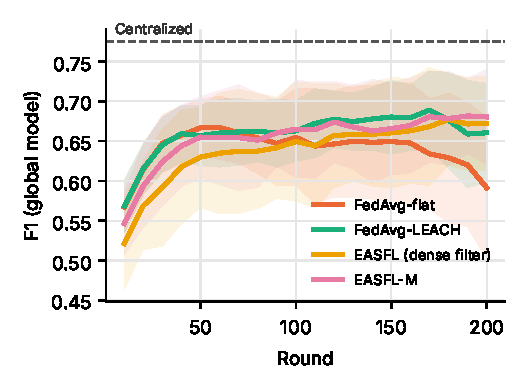
\includegraphics[width=\columnwidth]{figs/fig_convergence.pdf}
\caption{F1 of the global model during training (mean $\pm$ std, 5 seeds). FedAvg-flat degrades as its nodes die.}
\label{fig:conv}
\end{figure}

\subsection{Network Lifetime and Ablation}
Fig.~\ref{fig:alive} shows alive nodes over time and Table~\ref{tab:life} the lifetime milestones. EASFL delays the first node death to round 547, against 35 for FedAvg-LEACH (15.6$\times$) and 25 for centralized collection, and its HND (645) is 4.4$\times$ that of FedAvg-LEACH. Its characteristic ``plateau then cliff'' curve reflects balanced drain: no node dies until residual energies have been evened out.

\begin{figure}[t]
\centering
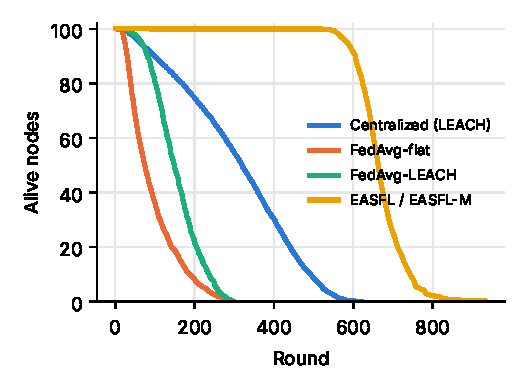
\includegraphics[width=0.92\columnwidth]{figs/fig_alive.pdf}
\caption{Alive nodes per round (mean of 5 seeds, 60 raw samples per node-round for centralized collection).}
\label{fig:alive}
\end{figure}

\begin{table}[t]
\caption{Lifetime (Rounds) and Energy in the First 200 Rounds}\label{tab:life}
\centering\footnotesize
\begin{tabular}{@{}lcccc@{}}
\toprule
Scheme / variant & FND & HND & LND & $E_{200}$ (J)\\
\midrule
Centralized (LEACH) & 25 & 320 & 489 & 25.9\\
Centralized (EA-CH) & 142 & 246 & 461 & 39.1\\
FedAvg-flat & 18 & 73 & 189 & 49.0\\
FedAvg-LEACH & 35 & 145 & 233 & 47.3\\
\textbf{EASFL} & \textbf{547} & 645 & 731 & \textbf{15.6}\\
\quad w/o participant selection & 317 & 538 & 628 & 19.4\\
\quad w/o compression & 219 & 248 & 291 & 40.9\\
\quad w/o energy-aware CH (LEACH) & 177 & \textbf{697} & \textbf{802} & 15.9\\
\bottomrule
\end{tabular}
\end{table}

\begin{figure}[t]
\centering
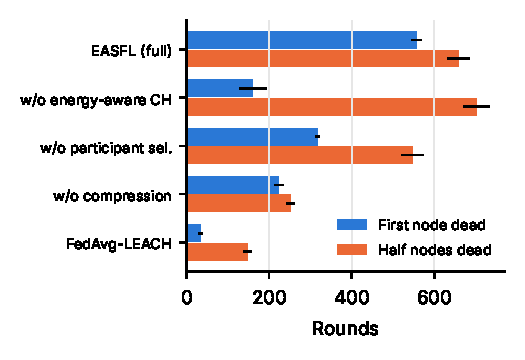
\includegraphics[width=0.92\columnwidth]{figs/fig_ablation.pdf}
\caption{Ablation: contribution of each EASFL component to lifetime (mean $\pm$ std).}
\label{fig:abl}
\end{figure}

The ablation (Table~\ref{tab:life}, Fig.~\ref{fig:abl}) isolates each component. Compression is the largest contributor: without it, energy use rises 2.6$\times$ and HND falls from 645 to 248. Participant selection adds 73\% to FND. Energy-aware CH selection triples FND (547 vs.\ 177) but slightly shortens HND and LND relative to LEACH rotation (645 vs.\ 697, 731 vs.\ 802). This is a genuine trade-off: deterministic selection favours nodes close to the BS and well connected, which equalizes early drain but concentrates the CH burden on a subset late in life. Applications that need full coverage (FND) should prefer the energy-aware score; those that tolerate gradual coverage loss may prefer rotation. The same trade-off appears when the energy-aware score is applied to centralized collection (FND 25 $\rightarrow$ 142, HND 320 $\rightarrow$ 246).

\subsection{Robustness to Poisoning}
Fig.~\ref{fig:pois} plots global-model F1 against the fraction of malicious nodes for the four attacks, and Table~\ref{tab:pois} details the 20\% case. Undefended FedAvg collapses under the scaled sign flip (F1 0.24 at 20\%, 0.13 at 30\%). With 10\% and 20\% attackers, EASFL keeps global F1 between 0.64 and 0.71 across all attacks, within 0.07 of its clean value (0.71) and higher than every compared aggregation rule in all eight cases. Removing EASFL's filtering and quarantine (``EASFL w/o robust'') lets the sign-flip attack succeed (0.18), confirming that the defence and not compression or participant selection provides the resilience. The label-flip attack is notable: its updates are neither large nor reversed in direction, yet EASFL (0.67) outperforms median (0.53) and trimmed mean (0.57), because repeated flags quarantine persistent offenders. Krum performs poorly throughout (0.35--0.52), even without attackers, because selecting a single update discards the information carried by heterogeneous nodes.

\begin{figure*}[t]
\centering
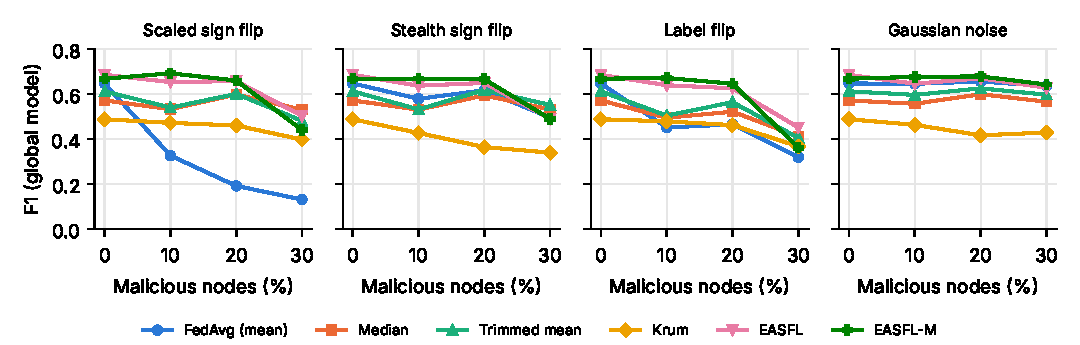
\includegraphics[width=0.95\textwidth]{figs/fig_poisoning.pdf}
\caption{Global-model F1 versus fraction of malicious nodes for four poisoning attacks (mean of 5 seeds).}
\label{fig:pois}
\end{figure*}

\begin{table}[t]
\caption{F1 With 20\% Malicious Nodes: Global Model / Personalized}\label{tab:pois}
\centering\scriptsize
\setlength{\tabcolsep}{3pt}
\begin{tabular}{@{}lcccc@{}}
\toprule
Defence & Sign flip & Stealth & Label flip & Gaussian\\
\midrule
FedAvg (mean) & 0.24 / 0.40 & 0.64 / 0.80 & 0.50 / 0.81 & 0.69 / 0.83\\
Median & 0.62 / 0.81 & 0.63 / 0.81 & 0.53 / 0.82 & 0.65 / 0.82\\
Trimmed mean & 0.60 / 0.80 & 0.65 / 0.81 & 0.57 / 0.82 & 0.68 / 0.83\\
Krum & 0.49 / 0.75 & 0.35 / 0.73 & 0.48 / 0.75 & 0.44 / 0.73\\
EASFL w/o robust & 0.18 / 0.41 & 0.66 / 0.81 & 0.43 / 0.82 & 0.70 / 0.82\\
EASFL w/o cosine & 0.70 / 0.81 & 0.66 / 0.80 & 0.65 / 0.82 & 0.70 / 0.82\\
\textbf{EASFL} & \textbf{0.70} / 0.82 & \textbf{0.67} / 0.81 & \textbf{0.67} / 0.82 & \textbf{0.71} / 0.82\\
\bottomrule
\end{tabular}
\end{table}

Two further observations matter for practice. First, personalization is itself a strong mitigation: after local fine-tuning, label-flip and Gaussian attacks barely affect any scheme. It does not, however, rescue the undefended schemes from the sign-flip attack (0.40), so robust aggregation remains necessary. Second, the defence has limits. At 30\% attackers EASFL becomes unstable across seeds (sign flip: F1 0.50 $\pm$ 0.25; stealth: 0.46 $\pm$ 0.21), whereas the coordinate-wise median degrades more gracefully (0.55 in both cases). We therefore claim resilience up to 20\% compromised nodes. The cosine test added little beyond the norm test and quarantine (Table~\ref{tab:pois}); it is cheap and retained, but its effect is not statistically distinguishable in our runs.

\subsection{Packet Loss}
With packet-loss probabilities from 0 to 0.3, EASFL's global F1 stays between 0.69 and 0.72 and its personalized F1 at 0.82, whereas FedAvg-LEACH's global F1 falls from 0.69 to 0.65 at 30\% loss. Because each round aggregates many small, independent uploads, isolated losses mainly reduce the effective participation rather than biasing the update.

\subsection{Sensitivity to the Synthetic Workload}
To verify that the conclusions are not artefacts of the generator settings, we varied the Dirichlet concentration $\alpha\in\{0.1,\dots,10\}$, the fault magnitude ($0.5$--$1.5\times$) and the anomaly rate ($0.5$--$2\times$). Fig.~\ref{fig:sens} shows that personalized EASFL matches or exceeds the centralized model in every setting except the smallest faults ($0.5\times$, where all methods reach only F1 $\approx0.54$ because faults are within noise), and stays within 0.02 of personalized FedAvg-LEACH throughout. Energy and traffic do not depend on the data, so EASFL's lifetime advantage is unaffected by these settings.

\begin{figure*}[t]
\centering
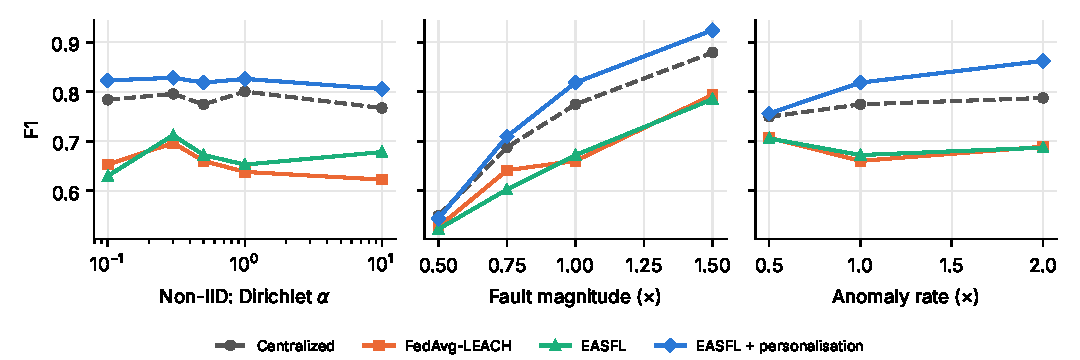
\includegraphics[width=0.95\textwidth]{figs/fig_sensitivity.pdf}
\caption{Sensitivity of F1 to the non-IID degree (Dirichlet $\alpha$), fault magnitude and anomaly rate (mean of 5 seeds).}
\label{fig:sens}
\end{figure*}

\subsection{When Is Centralized Collection Preferable?}
The energy of centralized collection grows with the raw sampling volume, whereas EASFL's communication does not. Varying the samples each node reports per round, centralized collection with LEACH achieves FND/HND of 81/1379 rounds at 10 samples, 45/589 at 30, 25/320 at 60 and 6/85 at 240. Hence, for very low reporting rates ($\le$10 samples per round) centralized collection outlives EASFL in HND, although its FND remains far shorter (81 vs.\ 547); above roughly 30 samples per round EASFL dominates on all lifetime metrics. The model size and the sampling rate together determine which design is preferable, and the cost model of Section~\ref{sec:model} allows this crossover to be computed before deployment.

\subsection{Validation on the Intel Lab Deployment}\label{sec:intel}
To test the conclusions on real sensor data, we replace the synthetic generator with the readings of the Intel Berkeley Research Lab deployment~\cite{intellab2004} and the random layout with its real mote coordinates. We use 28 Feb--9 Mar 2004, when 50--52 motes report, drop physically implausible readings, and keep the 50 motes with at least 300 gap-free windows of 10 samples (31\,s sampling). Per mote, 300 windows are spaced evenly over the period; the first 200 in time train and the last 100 test. The traces carry no expert labels, so the four fault types of Section~\ref{sec:model} are injected into the real windows with the same per-node rates and non-IID mixes, at amplitudes scaled by each mote's measured noise per channel. Detection therefore runs against real noise, diurnal cycles and lighting changes. The lab measures about $40.5\times31$\,m and the BS sits 75\,m beyond its edge, as in the synthetic layout; all other parameters are unchanged. Table~\ref{tab:intel} reports five seeds.

\begin{table*}[t]
\caption{Intel Lab Deployment (50 Motes, Real Readings and Layout, Injected Faults; Mean of 5 Seeds). \rev{--: Not Applicable or Not Measured in This Run}}\label{tab:intel}
\centering\footnotesize
\begin{tabular}{@{}lcccccccc@{}}
\toprule
Scheme & F1 global & F1 personalized & F1 network & Traffic (Mbit) & Energy (J) & Alive @200 & FND & HND\\
\midrule
Centralized (LEACH) & $0.543\pm0.021$ & $0.568\pm0.008$ & 0.516 & -- & 8.1 & 41 & 43 & 525\\
Local only & $0.406\pm0.035$ & $0.388\pm0.041$ & -- & 0 & -- & -- & -- & --\\
FedAvg-flat & $0.557\pm0.012$ & $0.559\pm0.026$ & $0.285\pm0.090$ & 110.1 & 23.3 & 17.6 & 81 & 174\\
FedAvg-LEACH & $0.556\pm0.022$ & $0.564\pm0.018$ & $0.321\pm0.046$ & 114.2 & 21.1 & 25.0 & 40 & 197\\
EASFL (dense filter) & $0.519\pm0.020$ & $0.530\pm0.034$ & $0.530\pm0.034$ & \textbf{7.1} & \textbf{6.4} & \textbf{50.0} & \textbf{619} & \textbf{803}\\
\textbf{EASFL-M} (mask-aware) & $\mathbf{0.561\pm0.009}$ & $\mathbf{0.567\pm0.019}$ & $\mathbf{0.567\pm0.019}$ & 7.2 & 6.5 & \textbf{50.0} & \textbf{619} & \textbf{803}\\
\quad w/o compression & $0.560\pm0.020$ & $0.559\pm0.027$ & $0.558\pm0.029$ & 72.4 & 16.9 & 49.0 & 239 & 310\\
\quad w/o robust filtering & $0.557\pm0.016$ & $0.554\pm0.023$ & $0.554\pm0.023$ & 7.2 & 6.5 & 50.0 & -- & --\\
\quad w/o participant selection & $0.520\pm0.020$ & $0.527\pm0.024$ & $0.527\pm0.024$ & 11.7 & 8.4 & 50.0 & 351 & 638\\
\bottomrule
\end{tabular}
\end{table*}

The energy and lifetime results carry over. EASFL transmits $16\times$ less traffic and uses $3.3\times$ less energy than FedAvg-LEACH over 200 rounds, keeps all 50 motes alive, and delays the first node death from round 40 to 619 and the half-network death from 197 to 803. Its network-level F1 (0.53) is the highest of all schemes, against 0.32 for FedAvg-LEACH and 0.52 for centralized collection, which has lost 9 motes by round 200.

Two results differ from the synthetic study. First, EASFL with the dense filter has a per-node F1 0.04 below FedAvg-LEACH (0.519 vs.\ 0.556). The ablation locates the cause: removing either compression or robust filtering restores it (0.560 and 0.557). On heterogeneous real nodes, honest updates with different top-$k$ supports fail the dense direction test, 4.0--8.1 honest nodes (mean over rounds, per seed) are in quarantine, and the coordinate-wise trimmed mean shrinks sparse coordinates. EASFL-M removes this loss (Section~\ref{sec:mask}): 0.561 per-node and 0.567 network-level F1, with no honest node quarantined. Second, on-node personalization gives little on real data (0.519 to 0.530, and no gain for the other schemes), unlike the 0.11 gain on the synthetic workload, so that gain should be read as workload-dependent.

Under 20\% malicious motes, undefended FedAvg-LEACH collapses under the scaled sign flip (F1 0.13), while EASFL keeps 0.43 (sign flip), 0.46 (stealth), 0.48 (label flip) and 0.51 (Gaussian), within 0.01--0.09 of its clean value; the sign-flip result varies widely across seeds ($\pm0.20$). Coordinate-wise median and trimmed mean on full-precision FedAvg-LEACH score 0.47--0.53, 0.02--0.04 higher than EASFL under every attack, but at $16\times$ the traffic, and Krum stays at 0.25--0.37. With the dense filter, EASFL's defence prevents collapse on compressed updates but does not outperform full-precision robust rules; Section~\ref{sec:mask} shows that the mask-aware variant closes this gap.

\subsection{Mask-Aware Robust Aggregation}\label{sec:mask}
Table~\ref{tab:mask} compares EASFL with the dense filter and with the mask-aware aggregation of Section~\ref{sec:method} (EASFL-M), against full-precision FedAvg-LEACH with coordinate-wise median and trimmed mean, at 20\% malicious nodes. Traffic and energy are identical for the two EASFL variants (7.2\,Mbit, 6.5\,J on Intel Lab), so lifetime is unchanged.

\begin{table}[t]
\caption{Global F1 With Dense and Mask-Aware Aggregation, Clean and With 20\% Malicious Nodes (Mean of 5 Seeds)}\label{tab:mask}
\centering\scriptsize\setlength{\tabcolsep}{3pt}
\begin{tabular}{@{}llccccc@{}}
\toprule
Data & Aggregation & Clean & Sign flip & Stealth & Label flip & Gauss\\
\midrule
Intel & FedAvg-LEACH (mean) & 0.556 & 0.13 & 0.49 & 0.45 & 0.55\\
 & FedAvg-LEACH median & -- & 0.47 & 0.47 & 0.52 & 0.51\\
 & FedAvg-LEACH trimmed & -- & 0.47 & 0.48 & 0.51 & 0.53\\
 & EASFL (dense) & 0.519 & 0.43 & 0.46 & 0.48 & 0.51\\
 & \textbf{EASFL-M} & \textbf{0.561} & \textbf{0.50} & 0.46 & \textbf{0.53} & \textbf{0.55}\\
\midrule
Synth. & FedAvg-LEACH (mean) & 0.706 & 0.24 & 0.64 & 0.50 & 0.69\\
 & FedAvg-LEACH median & -- & 0.62 & 0.63 & 0.53 & 0.65\\
 & FedAvg-LEACH trimmed & -- & 0.60 & 0.65 & 0.57 & 0.68\\
 & EASFL (dense) & 0.711 & 0.70 & 0.67 & 0.67 & 0.71\\
 & \textbf{EASFL-M} & 0.707 & \textbf{0.72} & \textbf{0.69} & 0.67 & 0.71\\
\bottomrule
\end{tabular}
\end{table}

On Intel Lab, EASFL-M raises clean per-node F1 from 0.519 to 0.561, above FedAvg-LEACH (0.556), and network-level F1 from 0.530 to 0.567. Under attack it improves on the dense filter by 0.04--0.07 for sign flip, label flip and Gaussian noise, and it matches or exceeds full-precision median and trimmed mean in three of four attacks while sending $16\times$ less traffic; the stealth attack remains 0.01--0.02 below them. On the synthetic workload the clean accuracy is unchanged (0.707, personalized 0.827), the 20\% results are equal or slightly higher, and with 10\% attackers EASFL-M is higher in all four attacks (0.70--0.72 vs.\ 0.64--0.68). With 30\% attackers both variants degrade and vary widely across seeds (EASFL-M 0.45--0.69), so we do not claim resilience beyond 20\%.

\subsection{Comparison With Matched Baselines}\label{sec:matched}
\rev{Table~\ref{tab:intel} and Table~\ref{tab:mask} compare EASFL with full-precision FedAvg, so part of each difference comes from compression and participation. To isolate the aggregation rule, we give every baseline EASFL's own top-10\% 8-bit compression with error feedback, energy-aware participant selection ($\rho=0.5$), energy-aware CH selection, 8-bit CH-to-BS and 16-bit broadcast. Only the aggregation differs: mean (FedAvg), coordinate median, trimmed mean (0.2), Krum, a support-aware median without filter or quarantine, EASFL with the dense filter, and EASFL-M. Traffic and energy are then the same for all rules (15.3\,Mbit and 15.4\,J over 200 rounds on the synthetic workload; 7.2\,Mbit and 6.4\,J on Intel Lab). Table~\ref{tab:matched} reports 20 seeds. Differences are tested on paired seeds with the Wilcoxon signed-rank test and Holm correction over the six comparisons in each setting; we also give 95\% bootstrap confidence intervals of the paired difference.

Without attack, EASFL-M is statistically equal to matched FedAvg and to the support-aware median on both data sets (differences 0.000--0.007). Coordinate median and Krum lose 0.12--0.29, because on sparse updates they count the zeros left by sparsification as votes. On Intel Lab the mask-aware rule improves on the dense filter by 0.038 (95\% CI [0.027, 0.048], $p<0.001$), confirming that the dense filter misreads honest heterogeneous updates. Under 20\% sign-flip attackers, EASFL-M is better than every matched baseline on both data sets: by 0.06--0.43 on the synthetic workload (Holm $p\le0.04$) and by 0.15--0.35 on Intel Lab (Holm $p\le0.003$). Under label flip it is better than mean, median and Krum, and equal to trimmed mean on Intel Lab. Under stealth and Gaussian attacks it equals the best matched baseline. With 30\% attackers (synthetic, 5 seeds) no rule is reliable; EASFL-M scores 0.45--0.69 with standard deviations up to 0.25, so we claim robustness only up to 20\%. The energy and lifetime gains of EASFL therefore come from compression, participation and CH selection, which a FedAvg baseline with the same settings shares; the aggregation rule contributes robustness under attack and on heterogeneous real data, not accuracy without attack. The 20-seed means are lower than the 5-seed values of Table~\ref{tab:mask} in some attack settings (e.g. synthetic sign flip $0.64\pm0.12$), which reflects seed-to-seed variability of the attacker set.}

\begin{table*}[t]
\caption{\rev{Global F1 With Matched Baselines: Same Compression, Participation and CH Policy for All Rules, 20\% Malicious Nodes in Attack Columns (Mean $\pm$ Std Over 20 Seeds)}}\label{tab:matched}
\centering\scriptsize\setlength{\tabcolsep}{2.6pt}
\begin{tabular}{@{}lccccc|ccccc@{}}
\toprule
 & \multicolumn{5}{c|}{Synthetic (100 nodes)} & \multicolumn{5}{c}{Intel Lab (50 motes)}\\
Aggregation & Clean & Sign flip & Stealth & Label flip & Gauss & Clean & Sign flip & Stealth & Label flip & Gauss\\
\midrule
Mean (FedAvg) & \pms{0.674}{0.041} & \pms{0.207}{0.086} & \pms{0.647}{0.068} & \pms{0.403}{0.056} & \pms{0.676}{0.046} & \pms{0.569}{0.035} & \pms{0.141}{0.061} & \pms{0.457}{0.072} & \pms{0.379}{0.102} & \pms{0.550}{0.036}\\
Coord.\ median & \pms{0.564}{0.060} & \pms{0.532}{0.069} & \pms{0.535}{0.064} & \pms{0.534}{0.068} & \pms{0.545}{0.067} & \pms{0.283}{0.097} & \pms{0.201}{0.113} & \pms{0.196}{0.104} & \pms{0.332}{0.069} & \pms{0.160}{0.094}\\
Trimmed mean & \pms{0.669}{0.069} & \pms{0.578}{0.127} & \pms{0.645}{0.065} & \pms{0.540}{0.101} & \pms{0.666}{0.062} & \pms{0.539}{0.029} & \pms{0.246}{0.128} & \pms{0.462}{0.055} & \pms{0.438}{0.085} & \pms{0.519}{0.029}\\
Krum & \pms{0.514}{0.106} & \pms{0.489}{0.122} & \pms{0.449}{0.111} & \pms{0.466}{0.122} & \pms{0.519}{0.115} & \pms{0.305}{0.087} & \pms{0.338}{0.096} & \pms{0.289}{0.104} & \pms{0.380}{0.085} & \pms{0.312}{0.102}\\
Support-aware median & \pms{0.676}{0.062} & \pms{0.572}{0.119} & \pms{0.664}{0.066} & \pms{0.537}{0.093} & \pms{0.685}{0.060} & \pms{0.570}{0.031} & \pms{0.271}{0.092} & \pms{0.467}{0.049} & \pms{0.435}{0.088} & \pms{0.548}{0.031}\\
EASFL, dense filter & \pms{0.672}{0.059} & \pms{0.614}{0.124} & \pms{0.647}{0.086} & \pms{0.606}{0.131} & \pms{0.657}{0.077} & \pms{0.532}{0.030} & \pms{0.422}{0.173} & \pms{0.470}{0.069} & \pms{0.483}{0.086} & \pms{0.513}{0.044}\\
\textbf{EASFL-M} & \pms{0.680}{0.059} & \pms{\textbf{0.639}}{0.118} & \pms{0.662}{0.063} & \pms{\textbf{0.610}}{0.113} & \pms{0.679}{0.053} & \pms{0.570}{0.032} & \pms{\textbf{0.486}}{0.156} & \pms{0.467}{0.057} & \pms{0.463}{0.152} & \pms{0.551}{0.032}\\
\bottomrule
\end{tabular}
\end{table*}

\subsection{Detection Over the Whole Network Lifetime}\label{sec:lifetimef1}
\rev{The results above stop learning at round 200, while the lifetime runs continue until the nodes are depleted. To show detection quality during the whole survival period, we continue learning every round until the network is dead and evaluate every 25 rounds (synthetic workload, 5 seeds; Table~\ref{tab:lifef1}). We include local-only learning, in which each node trains on its own data every round with the same per-round training energy as an FL participant and reports each flagged window to the BS in one packet. While nodes are alive, the live-node F1 of EASFL-M stays between 0.827 and 0.838 from round 200 to 800, so detection quality does not degrade; network-level F1 then falls only with coverage. Local-only learning detects less well (0.708 at round 200) but, because it never transmits model updates, it keeps 72\% of nodes alive at round 1000. Over rounds 1--500 EASFL-M has the highest cumulative network-level F1 (0.824 against 0.695 for local-only), but over rounds 1--1000 local-only is higher (0.631 against 0.551). This trade-off disappears when FL is used as a training phase: if all schemes train for 200 rounds and afterwards only detect and report alarms (the same accounting for every scheme), EASFL-M leads local-only at every horizon we evaluated (0.812 against 0.687 at round 500, 0.762 against 0.639 at round 1000 and 0.622 against 0.561 at round 2000). Matched FedAvg has the same lifetime curve as EASFL-M, consistent with Section~\ref{sec:matched}.}

\begin{table}[t]
\caption{\rev{Network-Level F1, Coverage and Cumulative Detection Over the Whole Lifetime With Learning Every Round (Synthetic, Mean of 5 Seeds)}}\label{tab:lifef1}
\centering\scriptsize\setlength{\tabcolsep}{1.5pt}
\begin{tabular}{@{}lccccc@{}}
\toprule
 & \multicolumn{4}{c}{Net F1 (coverage) at round} & Mean\\
Scheme & 200 & 400 & 600 & 800 & 1--1000\\
\midrule
Local only & 0.708 (1.00) & 0.685 (0.99) & 0.646 (0.95) & 0.547 (0.85) & 0.631\\
Centralized & 0.699 (0.75) & 0.380 (0.31) & 0 (0) & 0 (0) & 0.284\\
FedAvg-flat & 0.114 (0.08) & 0 (0) & 0 (0) & 0 (0) & 0.080\\
FedAvg-LEACH & 0.259 (0.23) & 0 (0) & 0 (0) & 0 (0) & 0.129\\
FedAvg, matched & 0.826 (1.00) & 0.831 (1.00) & 0.746 (0.82) & 0.027 (0.02) & 0.551\\
EASFL, dense & 0.821 (1.00) & 0.827 (1.00) & 0.666 (0.71) & 0.175 (0.10) & 0.567\\
\textbf{EASFL-M} & 0.827 (1.00) & 0.828 (1.00) & 0.741 (0.82) & 0.027 (0.02) & 0.551\\
\bottomrule
\end{tabular}
\end{table}

\section{Discussion and Limitations}
\textit{Synthetic and real data.} The synthetic workload provides exact ground truth and controllable heterogeneity, and the Intel Lab validation (Section~\ref{sec:intel}) tests the conclusions on real readings and a real layout. The energy, lifetime and network-level gains hold on both. On real data the dense filter cost 0.04 in per-node F1 because it misread honest sparsified updates; the mask-aware variant removes this loss and matches or exceeds full-precision robust rules in three of four attacks. Personalization gives little on real data, and the stealth attack remains slightly better handled by full-precision trimmed mean. The real traces carry no expert labels, so faults were injected; \rev{the Intel Lab experiment is therefore a semi-synthetic validation, and validation on traces with expert-labelled faults remains future work.}

\textit{Simulator scope.} The round-based simulator abstracts MAC contention, retransmissions, idle listening and sleep scheduling, which affect all schemes but may change absolute lifetimes. Training energy uses a fixed per-sample cost; on microcontrollers without floating-point units this cost can be higher, which would favour EASFL's participant selection further.

\rev{\textit{Where the gains come from.} Matched baselines (Section~\ref{sec:matched}) show that the energy and lifetime gains are due to compression, participation and CH selection, and that the mask-aware rule adds robustness under attack and on heterogeneous real data rather than clean accuracy.}

\textit{Threat model.} We assume honest CHs and non-colluding, non-adaptive attackers\rev{, and we claim robustness only up to 20\% malicious nodes.} Adaptive attacks crafted against the specific defence~\cite{fang2020}, backdoors~\cite{bagdasaryan2020} and compromised CHs remain open. EASFL provides integrity protection, not confidentiality; it can be combined with secure aggregation~\cite{bonawitz2017} at the cost of extra communication.

\section{Conclusion}
EASFL shows that federated anomaly detection can extend, rather than shorten, the life of a WSN when every protocol component is designed around radio energy. Compressed, selectively scheduled updates cut traffic by $13\times$ and energy by $3\times$ relative to hierarchical FedAvg and postpone the first node death by more than an order of magnitude; on-node personalization lifts per-node F1 above that of a centralized model without any radio cost; and two-tier robust aggregation with quarantine maintains accuracy with up to 20\% malicious nodes on the synthetic workload. Measured at the network level, where dead nodes cannot report anomalies, EASFL detects anomalies with F1 0.82 at round 200 while hierarchical FedAvg reaches 0.26. On real readings and the real layout of the Intel Lab deployment, EASFL keeps all 50 motes alive to round 200, and its mask-aware aggregation, which compares sparsified updates only on the coordinates they carry, reaches a per-node F1 of 0.56, on par with hierarchical FedAvg, while raising network-level F1 from 0.32 to 0.57. \rev{Compared with baselines given the same compression and participation, its mask-aware aggregation adds no accuracy without attack but is significantly more robust to sign-flip poisoning on both data sets, and its detection quality holds for the whole period in which nodes survive.} Future work will validate EASFL on traces with expert-labelled faults, harden the filter against stealthy norm-preserving attacks, extend the threat model to adaptive attackers and compromised CHs, and explore adaptive participation ratios driven by energy harvesting.

\section*{Acknowledgment}
The authors used Claude (Anthropic) to assist with the literature search and verification of reference metadata, with drafting and editing the text of the abstract, Related Work, the Intel Lab validation and the mask-aware aggregation (Sections~\ref{sec:intel} and~\ref{sec:mask}), and with writing the simulation code for those experiments\rev{, and, in this revision, with the matched-baseline and lifetime experiments (Sections~\ref{sec:matched} and~\ref{sec:lifetimef1}), their statistical analysis and the revised text}. The authors reviewed and verified all AI-assisted content, reran all reported experiments, and take full responsibility for the article.

\section*{Code Availability}
The simulator, experiment scripts, random seeds and raw results are publicly available at \url{https://github.com/vadlashiva/EASFL}.

\bibliographystyle{IEEEtran}
\bibliography{refs}

\end{document}
